\documentclass[]{article}
\usepackage{graphicx}
\usepackage{pdfpages}
\usepackage{adjustbox}
\usepackage[margin=1in]{geometry}
\usepackage{multicol}
\usepackage{amsmath}
\def\mathLarge#1{\mbox{\LARGE $#1$}}
\raggedright
\begin{document}


\title{HW 5}
\author{Nick Strayer}
\date{\today}
\maketitle

\begin{enumerate}
\item We have two sets to compare: Mk1s and MK2s....

\begin{adjustbox}{center}
\begin{tabular}{r|c|c}
   & Mk1 & Mk2 \\ \hline
n & 26,751 & 27,079\\
kills & 183  & 222 \\
\end{tabular}
\end{adjustbox}

We know that each BHK interaction occurred with one BHK and it isn't possible to lose more than one warrior per battle. There is a constant probability ($p$) of losing a warrior in a battle.  

\vspace{2em}
{\large Part a} 

A binomial distribution characterizes this data. A binomial distribution is the result from $n$ successive independent Bernoulli trials. A Bernoulli trial is characterized by a dichotomous result. In this case the warrior died, or the warrior lived, the chance of a success (or in this case of the warrior dying) is given by $p$. 

\vspace{2em}
{\large Part b} 

To the MCMCs!

Using MCMC per the in class coin flip problem we can compute the posterior distributions of the Mk1 and Mk2 kill rates (Problem\_1.py): 

\centerline{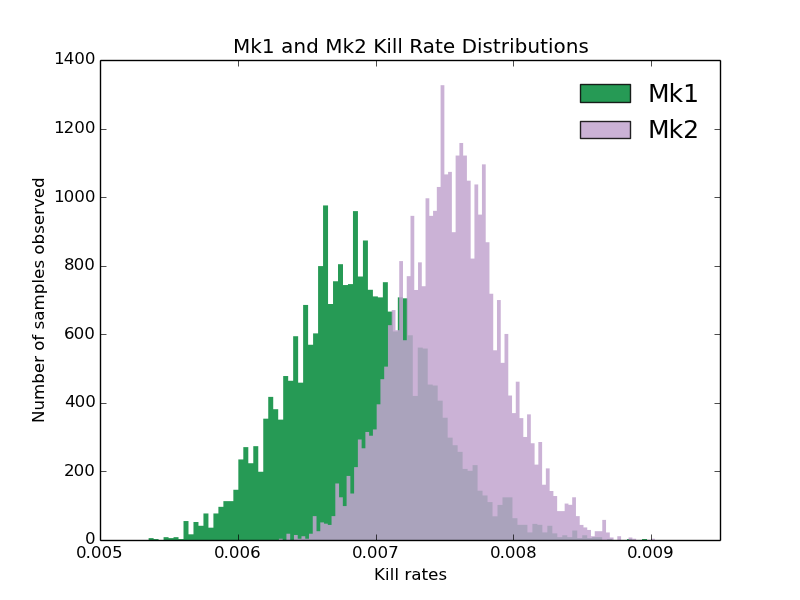
\includegraphics[scale = 0.6]{Mk1_Vs_Mk2.png}}

From this it is immediately apparent that there is a good amount of overlap between the two distributions. To further investigate this similarity we take the difference of the values given to us by MCMC in python (Problem\_1.py line 28). From this data we plot and check the middle 95\% of it to see if 0 is or isn't present:

\centerline{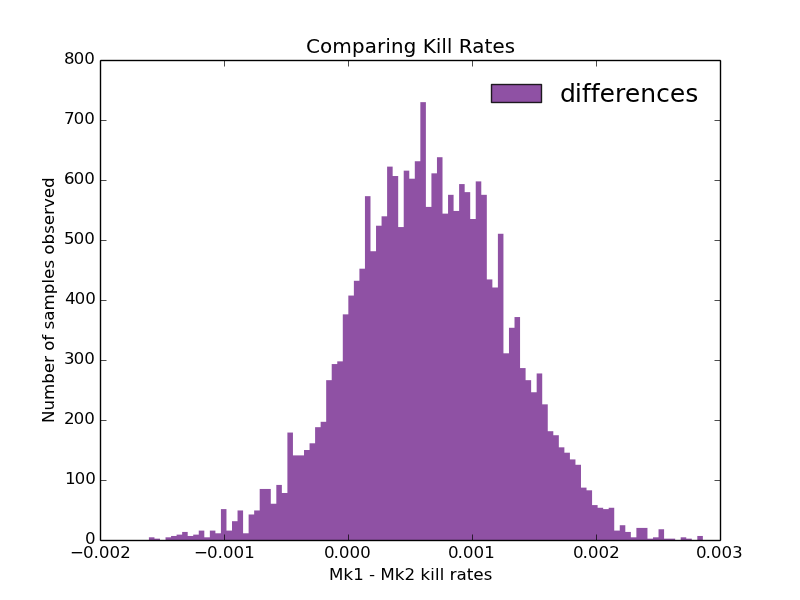
\includegraphics[scale = 0.6]{differences.png}}

The middle 95\% for this given run was [-0.000573233022814, 0.00192015873444]of which 0 is firmly entrenched. Furthermore, 0 sits at a percentile of 13.8 or a p-value of .138. Therefor \fbox{we fail to reject the null that there is no difference in rates.}

\vspace{1em}
{\large Bonus exact posterior plot!}


\centerline{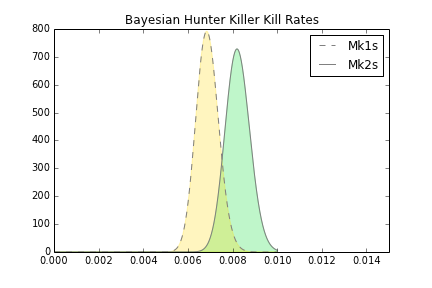
\includegraphics[scale = 0.6]{BHK_Plots.png}}

\newpage
\item {\large Part a} 

We observe convergence to the underlying distribution using MCMC by comparing plots of different amounts of iterations using the pymc algorithm (Problem\_2a.py): 

\vspace{1em}
\begin{adjustbox}{center}
\begin{tabular}{cc}
10,000 & 20,000 \\
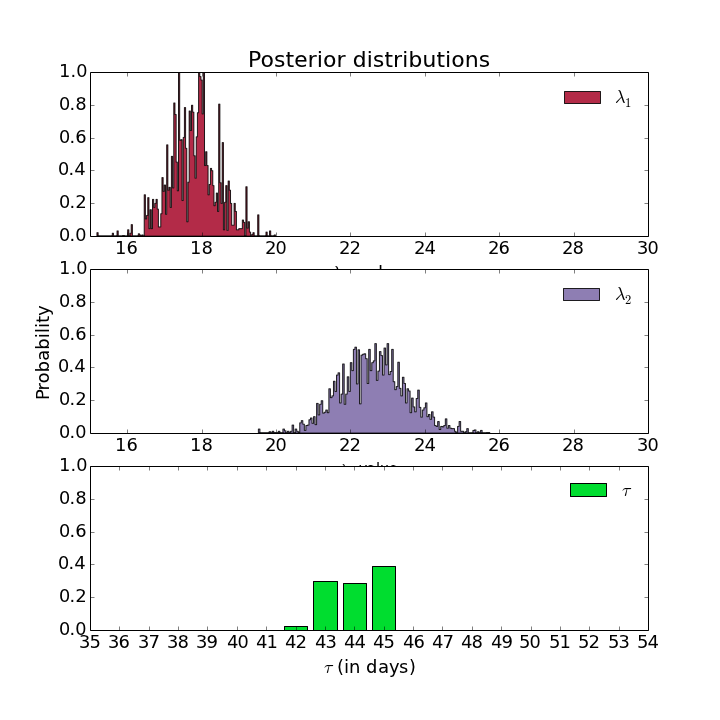
\includegraphics[scale = 0.22]{n_10000.png}  & 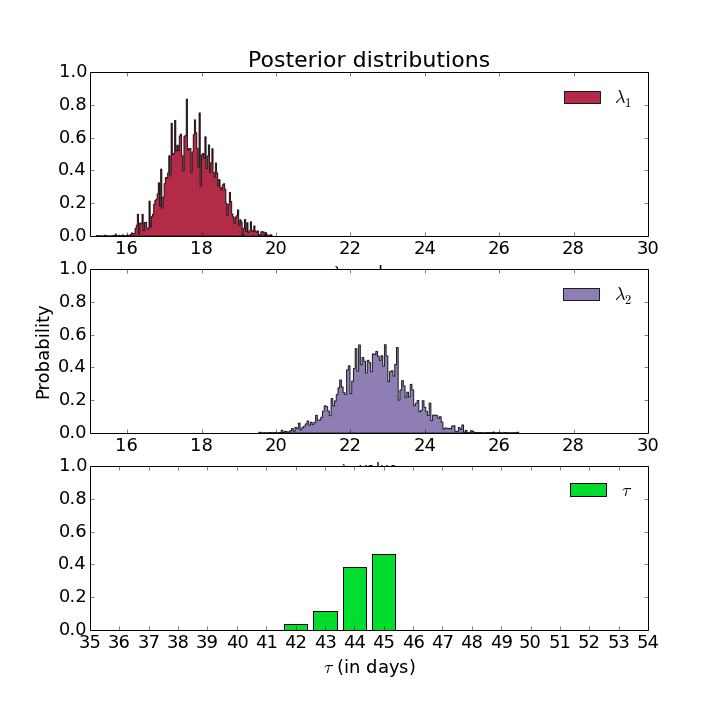
\includegraphics[scale = 0.22]{n_20000.png} \\
50,000 & 70,000 \\
 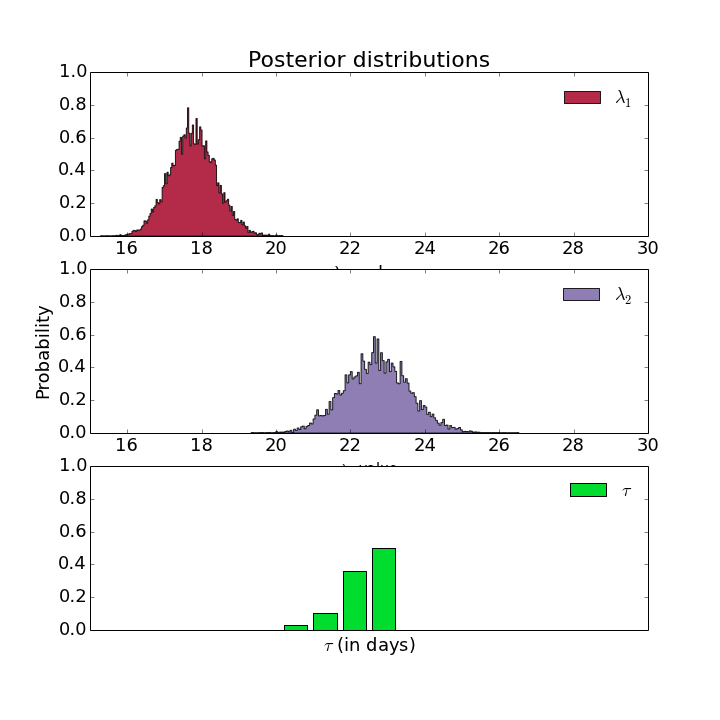
\includegraphics[scale = 0.22]{n_50000.png} & 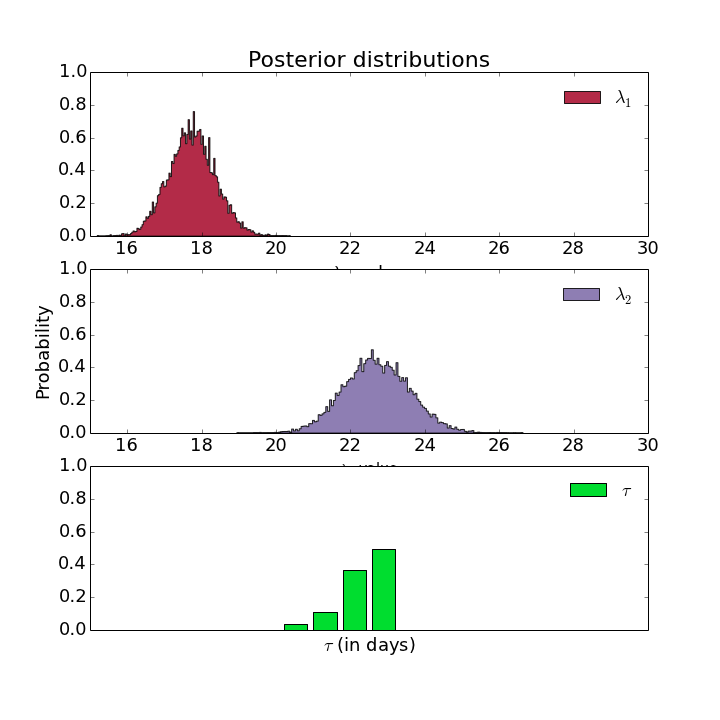
\includegraphics[scale = 0.22]{n_70000.png} \\
700,000 & \\
 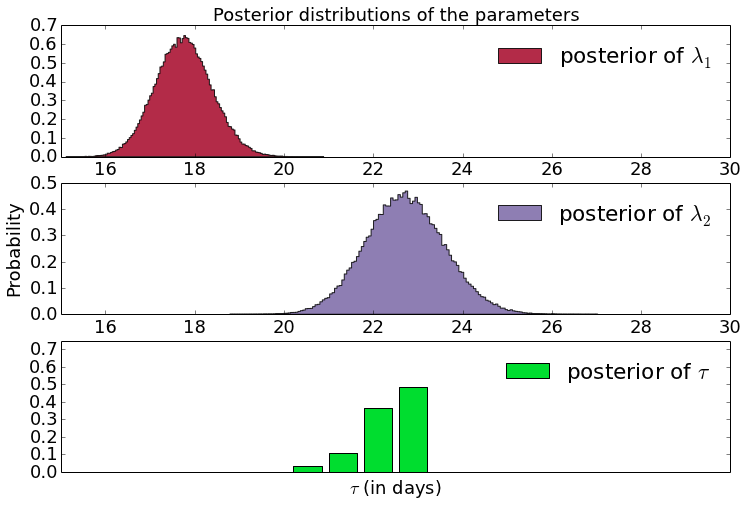
\includegraphics[scale = 0.22]{n_700000.png}  & \\
\end{tabular}
\end{adjustbox}

We can see from these plots that quickly the posteriors are converging to their underlying posteriors in a remarkably smooth way. 

\newpage
{\large Part b}  
\vspace{2em}

\begin{adjustbox}{center}
\begin{tabular}{lcl}
$ \Delta\lambda$ & = & $ \lambda_2 - \lambda_1$ \\
$f(t)$ & = &   $ \dfrac{ \Delta\lambda}{1+e^{-(\phi_1 + \phi_2 \cdot t)}} + \lambda 1$ \\
\end{tabular}
\end{adjustbox}

\vspace{2em}
$f(t)$ is a sigmoid function. I chose this because it fits with the instructions of "smoothly changes the poisson rate" very well. 
The $\lambda$s in this case represent the respective texting rates on either side of the transition. 
The $\phi$s combined to capture the behavior of the transition itself. The ratio $-\frac{\phi_1}{\phi_2}$ determines the actual point of transition and $\phi_2$ controls the steepness of the transition. 

\vspace{1em}
Upon updating the code from part a/class with the newly derived sigmoid function (see lines 26-34 in Problem\_2b.py) with priors for the $\phi$s being normals (lines 19,20) we run MCMC. 

\begin{multicols}{2}
\centerline{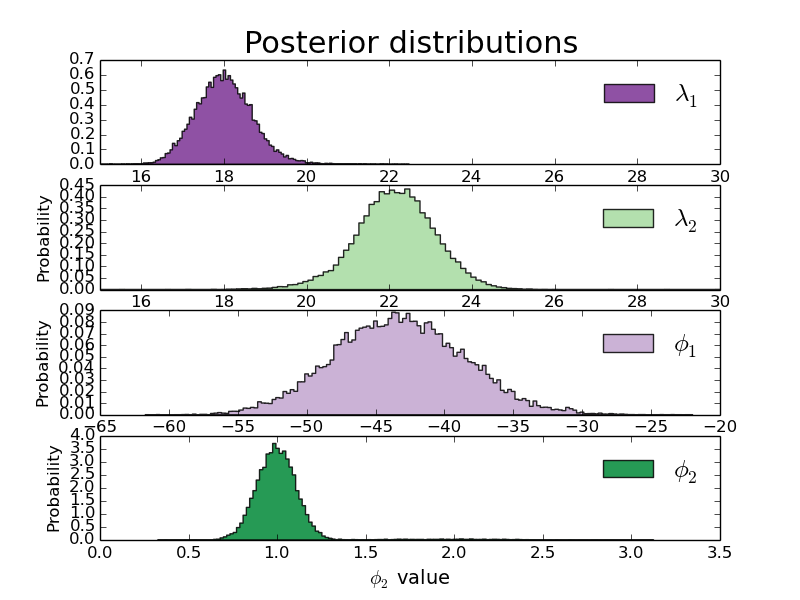
\includegraphics[scale = 0.4]{2b_final.png}}

\centerline{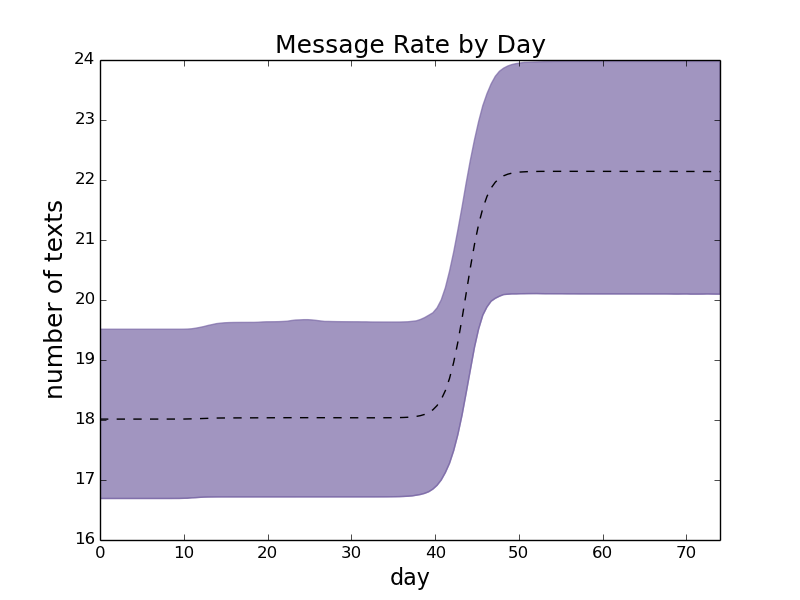
\includegraphics[scale = 0.4]{sigmoid_final.png}} 
\end{multicols}

We can plot the expected poisson rate for the texts over time (right figure) and arrive at the following figure (purple represents 95\% confidence interval):

Looking at results from the new model the shift to the higher rate happens very abruptly, even with the confidence intervals applied. This seems to imply that the new model is not necessarily better than the old. It is more complicated but most likely unnecessarily so. 

\end{enumerate}
\end{document}